\documentclass[journal,12pt,twocolumn]{IEEEtran}

\usepackage{setspace}
\usepackage{gensymb}
\singlespacing
\usepackage[cmex10]{amsmath}
\usepackage{amssymb}
\usepackage{xurl}

\usepackage{amsthm}
\usepackage{comment}
\usepackage{mathrsfs}
\usepackage{txfonts}
\usepackage{stfloats}
\usepackage{bm}
\usepackage{cite}
\usepackage{cases}
\usepackage{subfig}

\usepackage{longtable}
\usepackage{multirow}

\usepackage{enumitem}
\usepackage{mathtools}
\usepackage{steinmetz}
\usepackage{tikz}
\usepackage{circuitikz}
\usepackage{verbatim}
\usepackage{tfrupee}
\usepackage[breaklinks=true]{hyperref}
\usepackage{graphicx}
\usepackage{tkz-euclide}

\usetikzlibrary{calc,math}
\usepackage{listings}
    \usepackage{color}                                            %%
    \usepackage{array}                                            %%
    \usepackage{longtable}                                        %%
    \usepackage{calc}                                             %%
    \usepackage{multirow}                                         %%
    \usepackage{hhline}                                           %%
    \usepackage{ifthen}                                           %%
    \usepackage{lscape}     
\usepackage{multicol}
\usepackage{chngcntr}

\DeclareMathOperator*{\Res}{Res}

\renewcommand\thesection{\arabic{section}}
\renewcommand\thesubsection{\thesection.\arabic{subsection}}
\renewcommand\thesubsubsection{\thesubsection.\arabic{subsubsection}}

\renewcommand\thesectiondis{\arabic{section}}
\renewcommand\thesubsectiondis{\thesectiondis.\arabic{subsection}}
\renewcommand\thesubsubsectiondis{\thesubsectiondis.\arabic{subsubsection}}


\hyphenation{op-tical net-works semi-conduc-tor}
\def\inputGnumericTable{}                                 %%

\lstset{
%language=C,
frame=single, 
breaklines=true,
columns=fullflexible
}
\begin{document}


\newtheorem{theorem}{Theorem}[section]
\newtheorem{problem}{Problem}
\newtheorem{proposition}{Proposition}[section]
\newtheorem{lemma}{Lemma}[section]
\newtheorem{corollary}[theorem]{Corollary}
\newtheorem{example}{Example}[section]
\newtheorem{definition}[problem]{Definition}

\newcommand{\BEQA}{\begin{eqnarray}}
\newcommand{\EEQA}{\end{eqnarray}}
\newcommand{\define}{\stackrel{\triangle}{=}}
\bibliographystyle{IEEEtran}
\raggedbottom
\setlength{\parindent}{0pt}
\providecommand{\mbf}{\mathbf}
\providecommand{\pr}[1]{\ensuremath{\Pr\left(#1\right)}}
\providecommand{\qfunc}[1]{\ensuremath{Q\left(#1\right)}}
\providecommand{\sbrak}[1]{\ensuremath{{}\left[#1\right]}}
\providecommand{\lsbrak}[1]{\ensuremath{{}\left[#1\right.}}
\providecommand{\rsbrak}[1]{\ensuremath{{}\left.#1\right]}}
\providecommand{\brak}[1]{\ensuremath{\left(#1\right)}}
\providecommand{\lbrak}[1]{\ensuremath{\left(#1\right.}}
\providecommand{\rbrak}[1]{\ensuremath{\left.#1\right)}}
\providecommand{\cbrak}[1]{\ensuremath{\left\{#1\right\}}}
\providecommand{\lcbrak}[1]{\ensuremath{\left\{#1\right.}}
\providecommand{\rcbrak}[1]{\ensuremath{\left.#1\right\}}}
\theoremstyle{remark}
\newtheorem{rem}{Remark}
\newcommand{\sgn}{\mathop{\mathrm{sgn}}}
\providecommand{\abs}[1]{\vert#1\vert}
\providecommand{\res}[1]{\Res\displaylimits_{#1}} 
\providecommand{\norm}[1]{\lVert#1\rVert}
%\providecommand{\norm}[1]{\lVert#1\rVert}
\providecommand{\mtx}[1]{\mathbf{#1}}
\providecommand{\mean}[1]{E[ #1 ]}
\providecommand{\fourier}{\overset{\mathcal{F}}{ \rightleftharpoons}}
%\providecommand{\hilbert}{\overset{\mathcal{H}}{ \rightleftharpoons}}
\providecommand{\system}{\overset{\mathcal{H}}{ \longleftrightarrow}}
	%\newcommand{\solution}[2]{\textbf{Solution:}{#1}}
\newcommand{\solution}{\noindent \textbf{Solution: }}
\newcommand{\cosec}{\,\text{cosec}\,}
\providecommand{\dec}[2]{\ensuremath{\overset{#1}{\underset{#2}{\gtrless}}}}
\newcommand{\myvec}[1]{\ensuremath{\begin{pmatrix}#1\end{pmatrix}}}
\newcommand{\mydet}[1]{\ensuremath{\begin{vmatrix}#1\end{vmatrix}}}
\numberwithin{equation}{subsection}
\makeatletter
\@addtoreset{figure}{problem}
\makeatother
\let\StandardTheFigure\thefigure
\let\vec\mathbf
\renewcommand{\thefigure}{\theproblem}
\def\putbox#1#2#3{\makebox[0in][l]{\makebox[#1][l]{}\raisebox{\baselineskip}[0in][0in]{\raisebox{#2}[0in][0in]{#3}}}}
     \def\rightbox#1{\makebox[0in][r]{#1}}
     \def\centbox#1{\makebox[0in]{#1}}
     \def\topbox#1{\raisebox{-\baselineskip}[0in][0in]{#1}}
     \def\midbox#1{\raisebox{-0.5\baselineskip}[0in][0in]{#1}}
\vspace{3cm}
\title{ GATE Assignment 3}
\author{Savarana Datta - AI20BTECH11008}
\maketitle
\newpage
\bigskip
\renewcommand{\thefigure}{\theenumi}
\renewcommand{\thetable}{\theenumi}
Download all python codes from 
\begin{lstlisting}
https://github.com/SavaranaDatta/EE3900/tree/main/GATE Assignment3/codes
\end{lstlisting}
%
and latex codes from 
%
\begin{lstlisting}
https://github.com/SavaranaDatta/EE3900/tree/main/GATE Assignment3/main.tex
\end{lstlisting}

\section{Problem(GATE 1999(EC) 2.18)}
The Nyquist sampling frequency (in Hz) of a signal is given by 
\begin{align}
    6\times 10^{4} Sinc^{2}\brak{400t}+10^{6} Sinc^{3}\brak{100t} 
\end{align}is?
\begin{enumerate}
    \item 200
    \item 300
    \item 600
    \item 1000
\end{enumerate}
\section{Solution}
\begin{lemma}
\label{lem1}
Fourier transform of $sinc^{2}$ function 
\begin{align}
     sinc^{2}\brak{at} \fourier \frac{1}{|a|}tri\brak{\frac{f}{a}}\label{ft}
\end{align}
\end{lemma}
\begin{lemma}
\label{lem2}
Fourier transform of $sinc^{3}$ function 
\begin{multline}
     sinc^{3}\brak{at} \fourier \frac{1}{|a|} (3(a-f)^{2}sgn(f-a)-(f-3a)^{2}sgn(f-3a)\\-3(a+f)^{2}sgn(a+f)+(3a+f)^{2}sgn(3a+f))
\end{multline}
\end{lemma}
Using lemma \ref{lem1} 
\begin{align}
     X_{1}(f)=6\times 10^{4}sinc^{2}\brak{400t} \fourier 6\times 10^{4}\frac{1}{400}tri\brak{\frac{f}{400}}
\end{align}
$X_{1}(f)=0$ for $f>200Hz$
Using lemma \ref{lem2}
\begin{multline}
         X_{2}(f)=10^{6}\times sinc^{3}\brak{100t} \fourier 10^{6}\times\frac{1}{100} (3(100-f)^{2}sgn(f-100)-\\(f-300)^{2}sgn(f-300)-3(100+f)^{2}sgn(100+f)\\+(300+f)^{2}sgn(300+f))
\end{multline}
$X_{2}(f)=0$ for $f>300Hz$
Using the above equations, we have
\begin{multline}
    X(f) = \frac{6\times 10^{4}}{400}tri\brak{\frac{f}{400}}+ \frac{10^{6}}{100}(3(100-f)^{2}sgn(f-100)-\\(f-300)^{2}sgn(f-300)-3(100+f)^{2}sgn(100+f)+\\(3a+f)^{2}sgn(300+f))
\end{multline}
$X(f)$ is zero for $f>300Hz$
\begin{align}
    \text{Nyquist sampling frequency}&=2\times \text{ max frequency}\\
                       &=600Hz
\end{align}

\begin{figure}[!h]
 \centering
 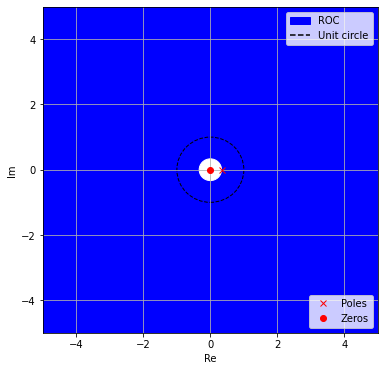
\includegraphics[width=\columnwidth]{fig1.png}
 \caption{Plot of x(t) sampled at 1kHz}
 \label{plot}
\end{figure}
\end{document}

